\chapter{Contexte et problématique}

	\addcontentsline{toc}{section}{Introduction}
	\section*{Introduction}
	\lettrine{D}{ans} ce chapitre de la première partie, nous présentons l'entreprise où nous avons effectué notre stage académique à savoir ITS. Nous parlerons ensuite du contexte relatif à notre sujet de stage de fin d'étude, nous terminerons par une mise en évidence de la problématique lié à ce contexte  et les objectifs à atteindre. 
	

	%Presentation de l'entreprise
	\section{Présentation de l'entreprise}
		\subsection{Historique}
			ITS  est une entreprise spécialisée dans la protection de l’information, la
sécurité informatique et la cryptologie de droit camerounais dont le siège générale se trouve à Yaoundé-Cameroun BP : 8570. Elle commence ces services depuis 2008.
		
		\subsection{Organisation générale}
		
		
		\subsection{Missions}
		
		\subsection{Services et Produits}
			Entreprise ITS renferme plusieurs services et une centre de formations:
				\subsubsection{Sévices}
					Les services sont :
						\begin{itemize}
							  \item Sécurité des S.I.
       						  \item Investigation Numériques
       						  \item Audit des S.I
     						  \item Gouvernance des SI
						\end{itemize}
				\subsubsection{E-Services}
					Dans les e-services on a plusieurs catégories :
					\begin{enumerate}
						\item \textbf{Web conférences:} rencontre internationale de Yaoundé sur la gestion du secret, l'usage de la cryptographie (Science du secret) dans la protection de l'information stratégique, la maîtrise des méthodes, moyens et systèmes de protection de l'information.
						\item \textbf{Web séminaires}
							\begin{itemize}
								\item \textbf{webinaire\footnote{Webinaire est un mot-valise associant les mots web et séminaire, créé pour désigner toutes les formes de réunions interactives de type séminaire faites via internet généralement dans un but de travail collaboratif ou d'enseignement à distance} Protection d'informations stratégiques :} Cette formation a pour objectif, la maîtrise des techniques de sécurisation et protection des informations stratégiques, ainsi que l'étude des mécanisme de protection de donnés sensibles.
								\item \textbf{webinaire : Audit informatique :} Le but de la formation est la maîtrise des notions et techniques d'audit des systèmes d'information, ainsi que l'étude des cas selon une démarche spécifique.
							\end{itemize}
                		\item Web consultations
        				\item E-Catalogue
                
					\end{enumerate}
    
				\subsubsection{Formations}
					Le centre de formation ITS est un centre de formation de référence spécialise dans les modules de formation suivants:
					\begin{itemize}
						\item sécurité des système d'information;
						\item investigations numériques;
						\item audit des systèmes d'information;
						\item gouvernance des systèmes d'information;
						\item développement informatique;
						\item infographie.
					\end{itemize} 
        Les formations ont un cycle de douze mois soit neuf mois de cours et trois mois de pratique en entreprise. Le centre de formation CF-ITS est agrée par le MINEFOPE(Ministère de l'Emploi et de la Formation Professionnelle) et donc délivre les certificats de fin de formation conformément à la réglementation en vigueur. En marge des formation dans les salles. \\
        
         Le centre donne l'accès gratuit et illimité aux forums et discussions via le portail web linkedin(www.linkedin.com) avec un nombre illimité d'experts internationaux du domaine de la cybercriminalité, cybersécurité, et investigation numériques, gouvernance et audit des systèmes d'information.
         
        		\subsubsection{Certifications}
        		
        		ITS offre également des certifications suivantes :
        			\begin{enumerate}
        				\item Certification Professionnelle Nationale (MINEFOP)
        					\begin{itemize}
        						\item Sécurité des systèmes d’Informations
								\item Investigations numériques
								\item Audit des systèmes d’information
								\item Gouvernance des systèmes d’information
        					\end{itemize}
                		\item Certification Professionnelle Internationale (ISACA)
                			\begin{itemize}
                				\item CISM - Certified Information Security Manager
								\item CISA - certified Information Systems Auditor
								\item CRISC - Certified in Risk and Information Systems Control
								\item CGEIT-Certified in Governance of Enterprise IT
                			\end{itemize}
                		\item Certification Professionnelle Internationale (CISCO)
        			\end{enumerate}
				
				\subsubsection{Produits}
					L'entreprise a mis à la disposition de tout le monde des logiciels open source, on peut citer entre autre les logiciels suivants :
					\begin{itemize}
						\item Utilitaire de désinstallation d'antivirus \textbf{AVAST},
						\item Logiciel de calcul de l'empreinte numérique des fichiers,
						\item Calcul du hash code des fichier par \textbf{MD5},
						\item Logiciel d'\textbf{EBIOS},
						\item Logiciel de stéganographie,
						\item \textbf{Ntop} - Logiciel de \textbf{monitoring} du réseau.
					\end{itemize}
					
					et des logiciels payants :
					\begin{itemize}
						\item Logiciel de récupération de mots de passe,
						\item et autres à venir.
					\end{itemize}
			
		
		\subsection{Cadre de stage}
			On a effectué notre stage au sein de la direction général de l'entreprise, elle se trouve dans le quartier \textbf{Biyem-Assi} dans la ville de Yaoundé, département de Mfoundi plus précisément situé en plein cœur du 6e arrondissement. Leur direction se trouve dans l'\textbf{Avenue Biyem-Assi} à côté de \textbf{Pharmacie Les Béatitudes}.\\
		
		%\begin{minipage}{\textwidth}
			\subsubsection{Situation géographique}
			La figure ci-dessous présente l’emplacement de notre lieu de stage réalisé grâce au service du géant Google  \textbf{Google Map}.
				\begin{figure}[h]
					\centering
					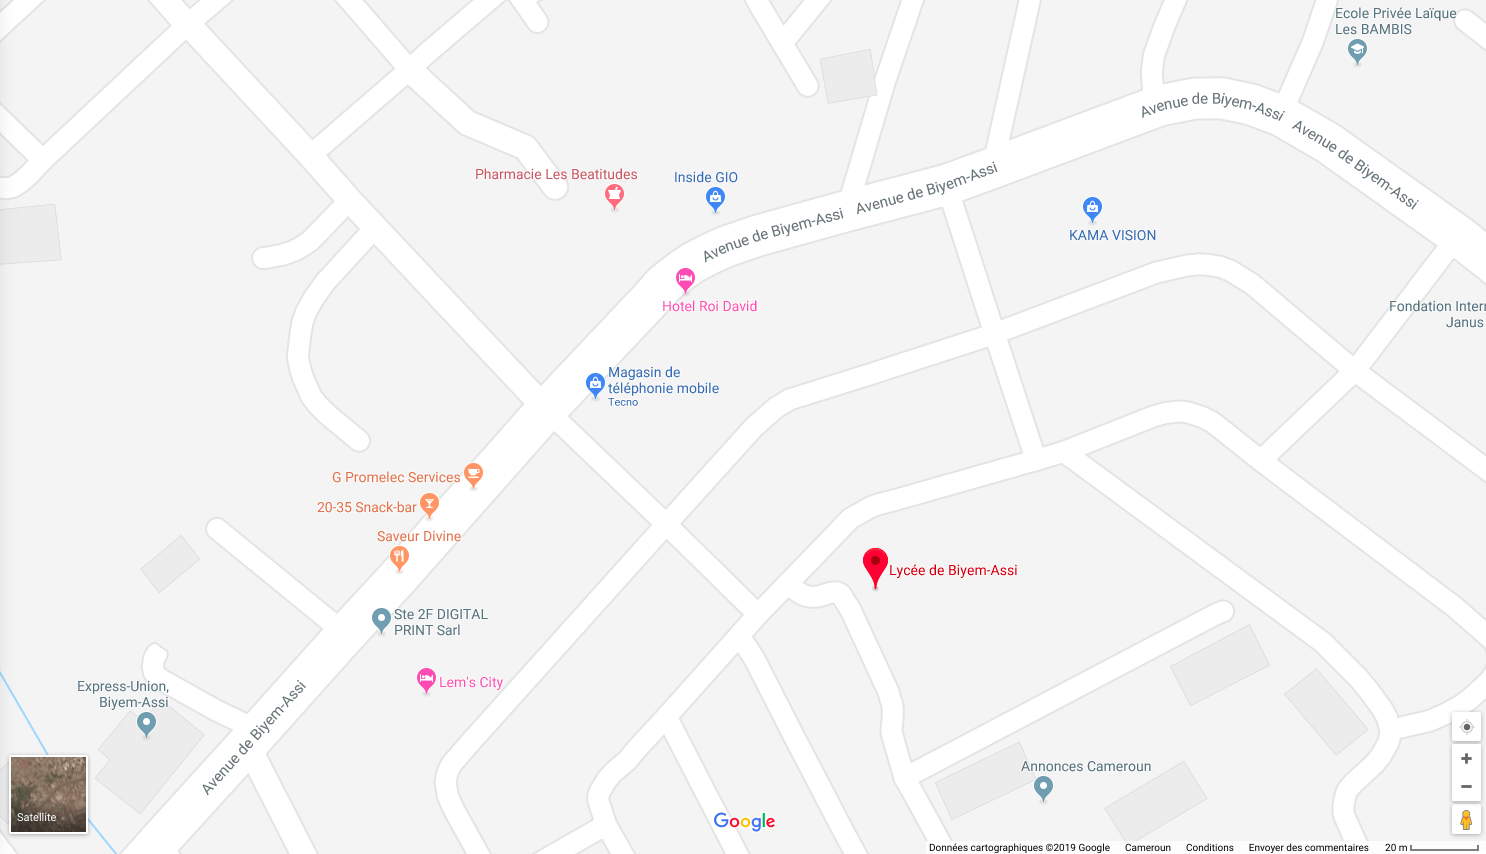
\includegraphics[scale=0.3]{../imgs/cartemap}
					\caption{Situation géographique du lieu de stage}
					\label{fig1}
			\end{figure}
		%\end{minipage}
			
	\section{Contexte}
	
	\section{Problématique}
	
	\section{Objectifs}
	
		\subsection{Objectif général}
		
		\subsection{Objectif spécifique}
		
	\section{Méthodologie}
	
	%\addcontentsline{toc}{section}{Conclusion}
	\section*{Conclusion}
